\subsection[Agents]{Agents $^{\star,\circ}$}\label{arc:agents}
This section presents the basic behaviour of our agents given the actions that all agents share.
Every agent team in the MAPC Scenario consists of 28 agents.
These agents are divided into five roles, the Explorer agent, the Repairer agent, the Saboteur agent, the Sentinel Agent and the Inspector agent (see \autoref{fig:arc:roles} from the MAPC Scenario).
There are six agents of each role except the Explorer agent role of which there are four agents.
Every agent role has some common and unique abilities.
The use and embodiment of these unique abilities into the agent role specific behaviour is explained in \autoref{alg:agentstrategies}.
All agents share the ability to execute the actions \texttt{skip}, \texttt{goto}, \texttt{survey}, \texttt{buy} and \texttt{recharge}.
\begin{description}
   \item[skip] The \texttt{skip} action is used as a last resort if there is nothing else for an agent left to do.
               This can be the case e.g. when an agent is occupying a vertex to form a zone, has full energy and health and is not endangered by an enemy.
               Such a situation happens seldom.
   \item[goto] The \texttt{goto} action is used to traverse over edges from one vertex to another adjacent vertex.
               Said traversing is only possible when the costs of the edge to traverse are lower than or equal to the energy the agent currently has.
               Else, the execution of the method will fail.
               By successfully executing the \texttt{goto} action, the current energy of the agent is reduced by the traversing costs of the edge.
   \item[survey] When the ability \texttt{survey} is executed, weights of edges in the visibility range of the agent are retrieved.
                 The count of edge weights an agent gets as percept is determined randomly based on the visibility range of the agent.
   \item[buy] With the action \texttt{buy} an agent is able to upgrade its values like maximum health, visibility range or in the case of the Saboteur agent strength.
   \item[recharge] If an agent has a low energy level the ability \texttt{recharge} fills up the energy of the agent.
                   By each \texttt{recharge} action the current energy is recharged by half of the maximum energy.
\end{description}

Besides the abilities each agent role set apart from each other by their visibility range, their maximum health and their maximum energy.
The saboteur agent has also a strength value, because it is the only agent which can attack enemy agents.
\begin{figure}[ht]
  \centering
  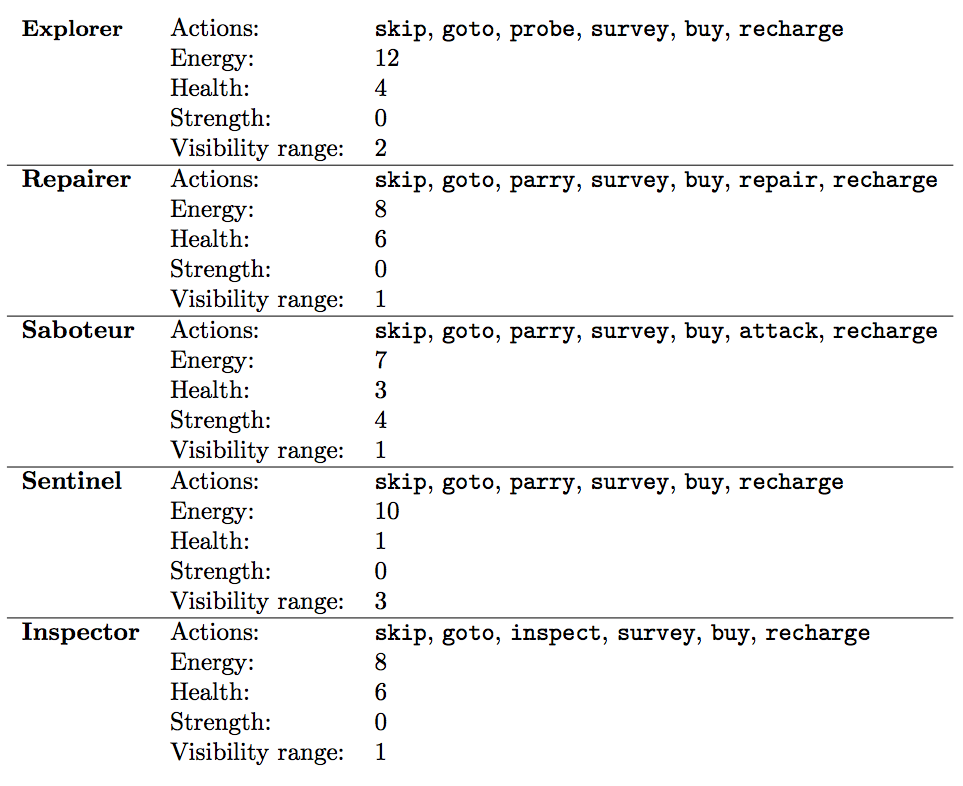
\includegraphics[width=0.9\linewidth]{images/roles.png}
  \caption{The different agent roles in the MAPC scenario.}
  \label{fig:arc:roles}
\end{figure}

Basically all agents were used for exploration, but we used for each role other priorities.
The highest priority was always to use the role defining ability if applicable.
For example if the Saboteur agent could attack any enemy agent, it attacks.
If an repairer agent could repair some damaged agent from our team, it repaired.
If the highest priority action was not applicable and the agents tried to explore the map (see \autoref{alg:exploration}).
Each agent decided which action to do autonomously based on the information it got from the map component or its percepts.

\subsection[Simulation Phases]{Simulation Phases$^{\star}$}\label{arc:simulation}
Our general strategy approach for the simulation was to use two phases, the exploration phase and the zoning phase.
In the exploration phase we tried to explore the map as quickly and complete as possible.
We distinguished three group types of exploring agents.
The first group consisted only of Explorer agents.
Their highest priority was to get vertex values by probing in an efficient way (see \autoref{alg:agentstrategies}).
Secondarily they used the \texttt{survey} action to explore the map only if they came across unsurveyed vertices.
They were not actively searching for or going to not surveyed vertices.
The second group was comprised of Saboteur agents.
We followed a very aggressive strategy and aimed to attack and disturb the enemy as much as possible, so we did not want to distract our Saboteur agents by exploring the map.
Saboteur agents would only explore the map if they did not know of an active enemy somewhere on the already explored map.
This strategy was followed by the Saboteur agents throughout the whole simulation.
The third and last group consisted of the remaining agents, which were the Repairer agents, the Sentinel agents and the Inspector agents.
These agents were used mainly for exploring the map.
They were coordinated by querying the map component for the next unexplored map area.
If they came to a vertex which edge weights to neighbour vertices were unknown, they used the survey action to get the information as percepts.
This weights were then passed to the map component and they repeated the exploring, by querying for the next not surveyed vertex and going there.
To prevent multiple agents from going to the same vertex and exploring the same area the map component used internally a locking mechanism.
We did not need a full coverage of the map, so we decided to remove every agent from the exploring agent team which could not be assigned a not surveyed vertex and put them in the zoning agent team.
By this we prevented agents from doing nothing and just idling around.
In the zoning phase all agents from the zoning agent team were used.
This included the Explorer agents but excluded the Saboteur agents, because they were following their own aggressive strategy.
For a detailed description of the zoning phase see \autoref{alg:zoning}.

